The viability of the proposed control structure is validated in the Aalborg University Smart Water Infrastructure Laboratory (SWIL). This modular laboratory consists of a number of units pumping units (PU), consumer units (CU), and piping units (PiU) that can be used for small-scale emulation of a real WDN.

\begin{figure}[h!]
	\includegraphics[height=4cm, width=\linewidth]{Graphics/SWIL.pdf}
	\caption{Picture of the AAU SWIL}
	\label{fig:AAUSWIL}
\end{figure}

The network topology in \cref{fig:WDNModel} is emulated via two PUs, a CU with two adjustable one-way valves each emulating a consumer, and a CU with an open bidirectional valve acting as the EWR, interconnected via two PiUs. Geodesic heights are emulated by pressuring the CUs. Experiments run for $12$ hours, with consumer demand curves based on real data and compressed to a fundamental frequency of $4$ hours such that each experiment corresponds to $3$ days. The controller attempts to follow a constant level reference throughout, starting $15 \si{mm}$ beneath it. After $4$ hours, a system leakage is simulated by fully opening the consumer valves for $30$ seconds. After $8$ hours, $50\%$ packet loss is introduced in the outer loop, which operates on a simulated TOD protocol. The tank level is seen on \cref{fig:OuterLoop}, while a snapshot of pump behaviour is seen on \cref{fig:InnerLoop}. The disturbance estimation scheme and true consumer flows can be seen on \cref{fig:DisturbanceEstimation}, with a zoomed-in view around the leakage seen on \cref{fig:Leakage}.

%We first present results pertaining to the VF-LQR. The controller is tested against nominal conditions, a variety of non-nominal time constants, and against a constant output disturbance. In each case the controls are clamped corresponding to the provided pump curves \cite{GrundfosDatablad}, the system is subjected to a varying state disturbance, and a sampling time of $t_s = 10\si{min}$ is assumed. The results can be seen on \cref{fig:LQRTracking}, displaying good tracking performance in each case; the disturbance is completely rejected, and the system tracks the reference. In all cases $Q = \left(\tilde{C}^T\tilde{C}\right)$ and $R = \text{diag}(0.1)$; the former guarantees an exponentially stable closed-loop system \cite{Liberzon2012}.


\begin{figure}[h!]
	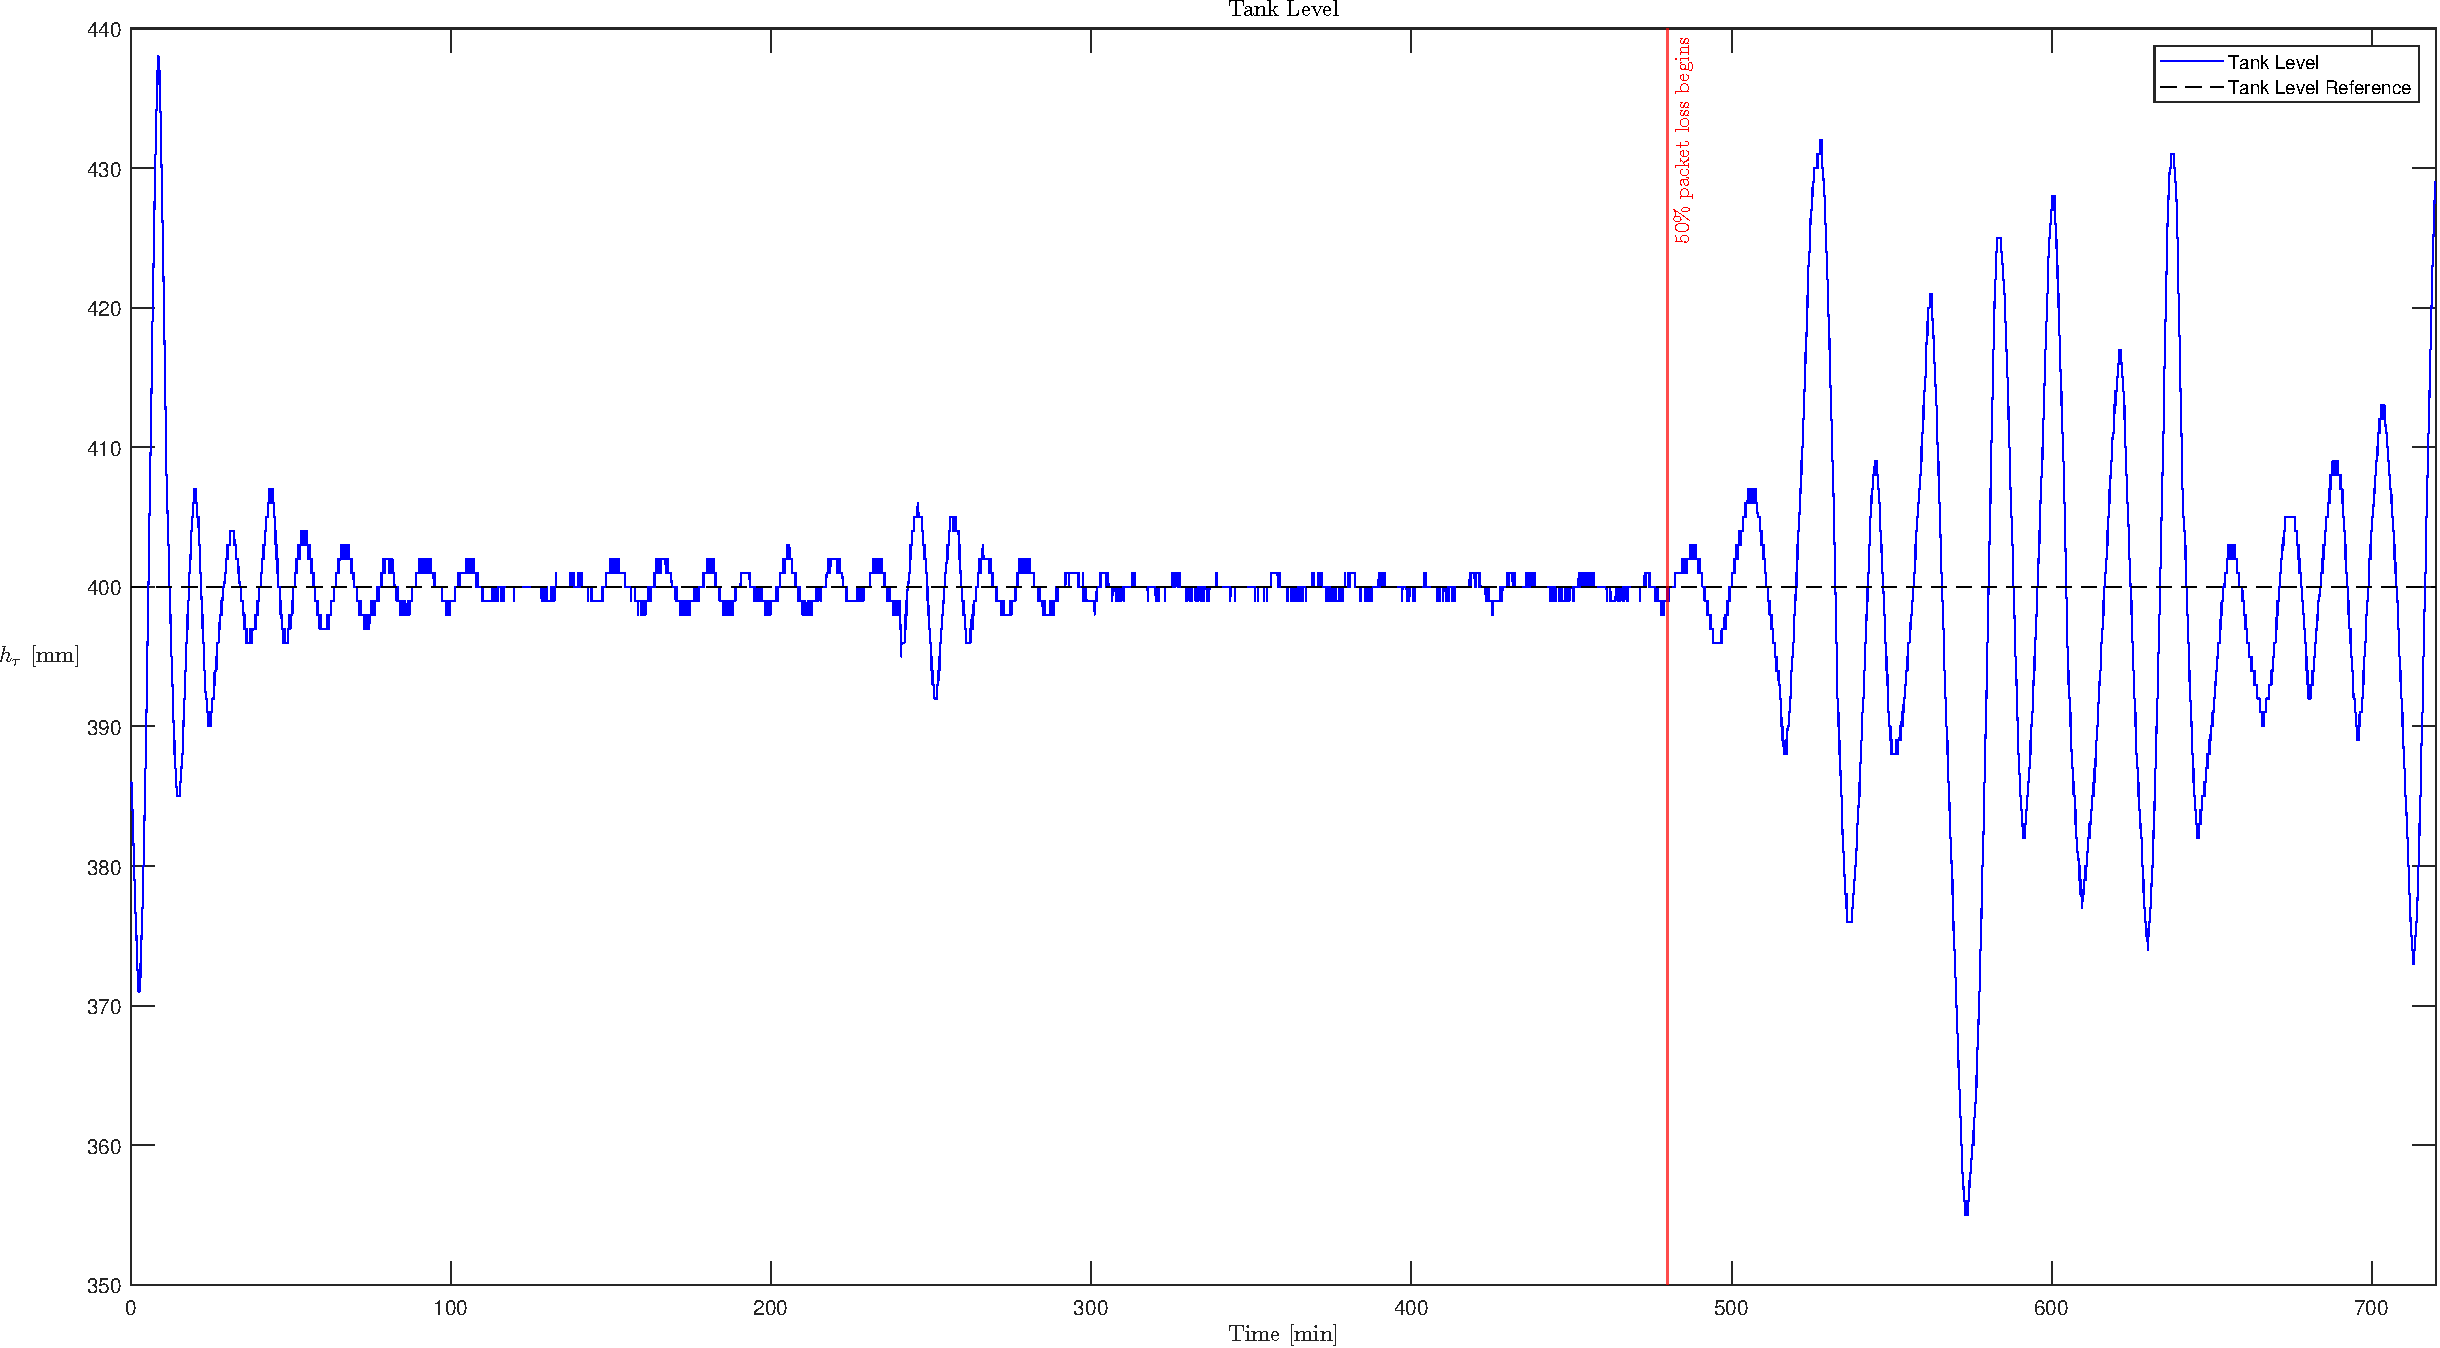
\includegraphics[height=4cm, width=\linewidth]{Graphics/OuterLoop.pdf}
	\caption{Outer loop.}
	\label{fig:OuterLoop}
\end{figure}


\begin{figure}[h!]
	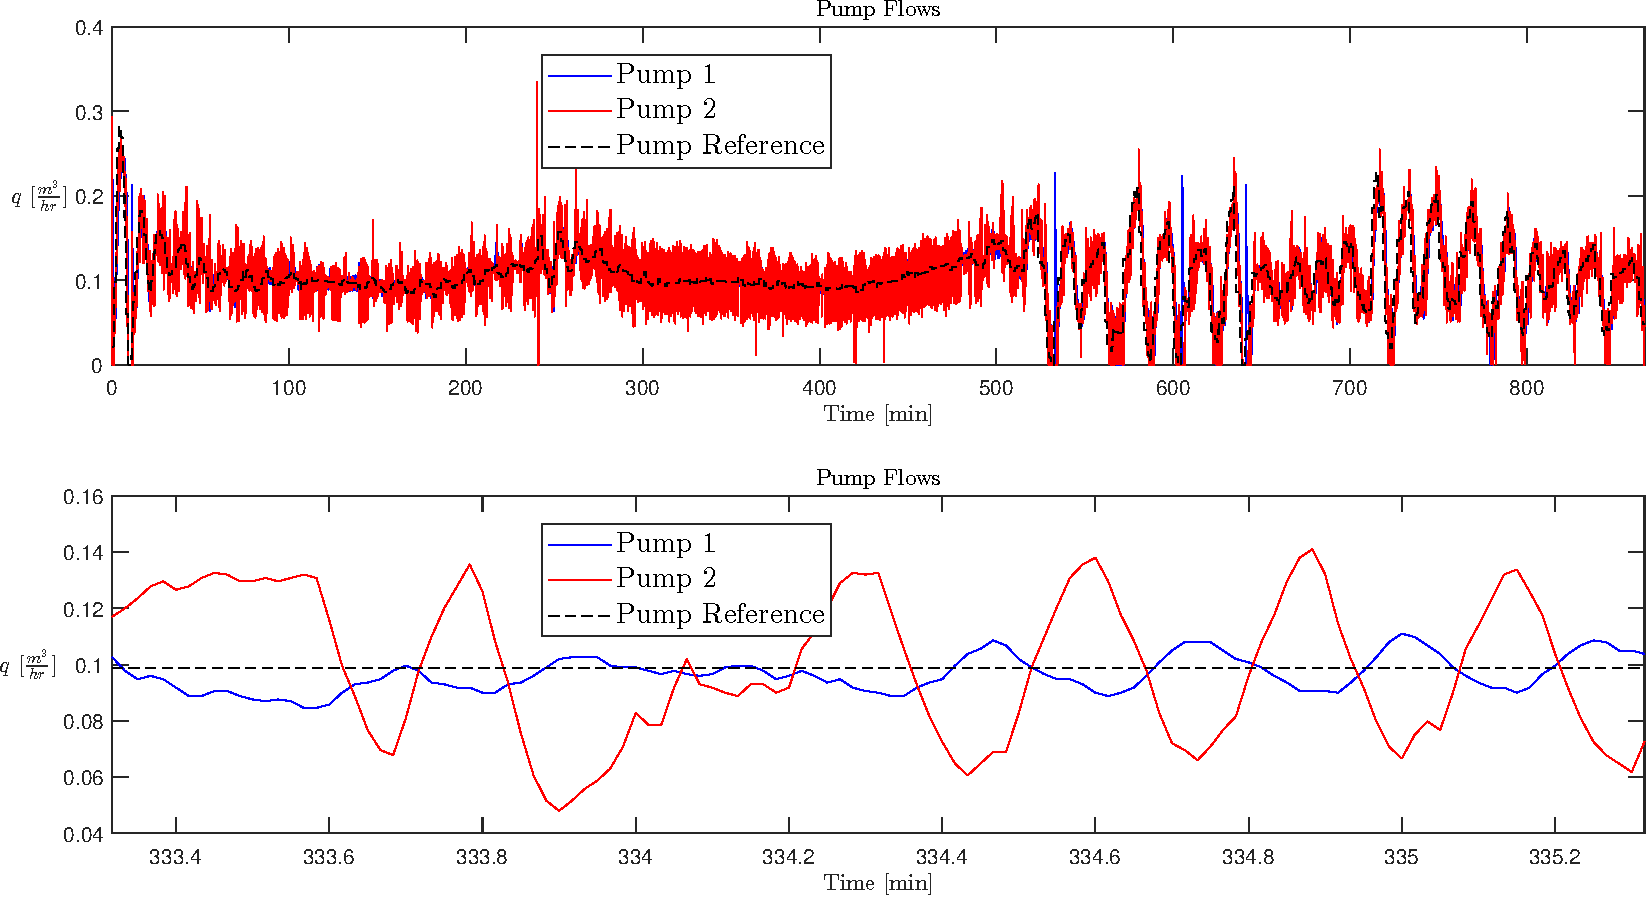
\includegraphics[width=\linewidth,height=4cm]{Graphics/InnerLoop.pdf}
	\caption{Inner loop.}
	\label{fig:InnerLoop}
\end{figure}


\begin{figure}[h!]
	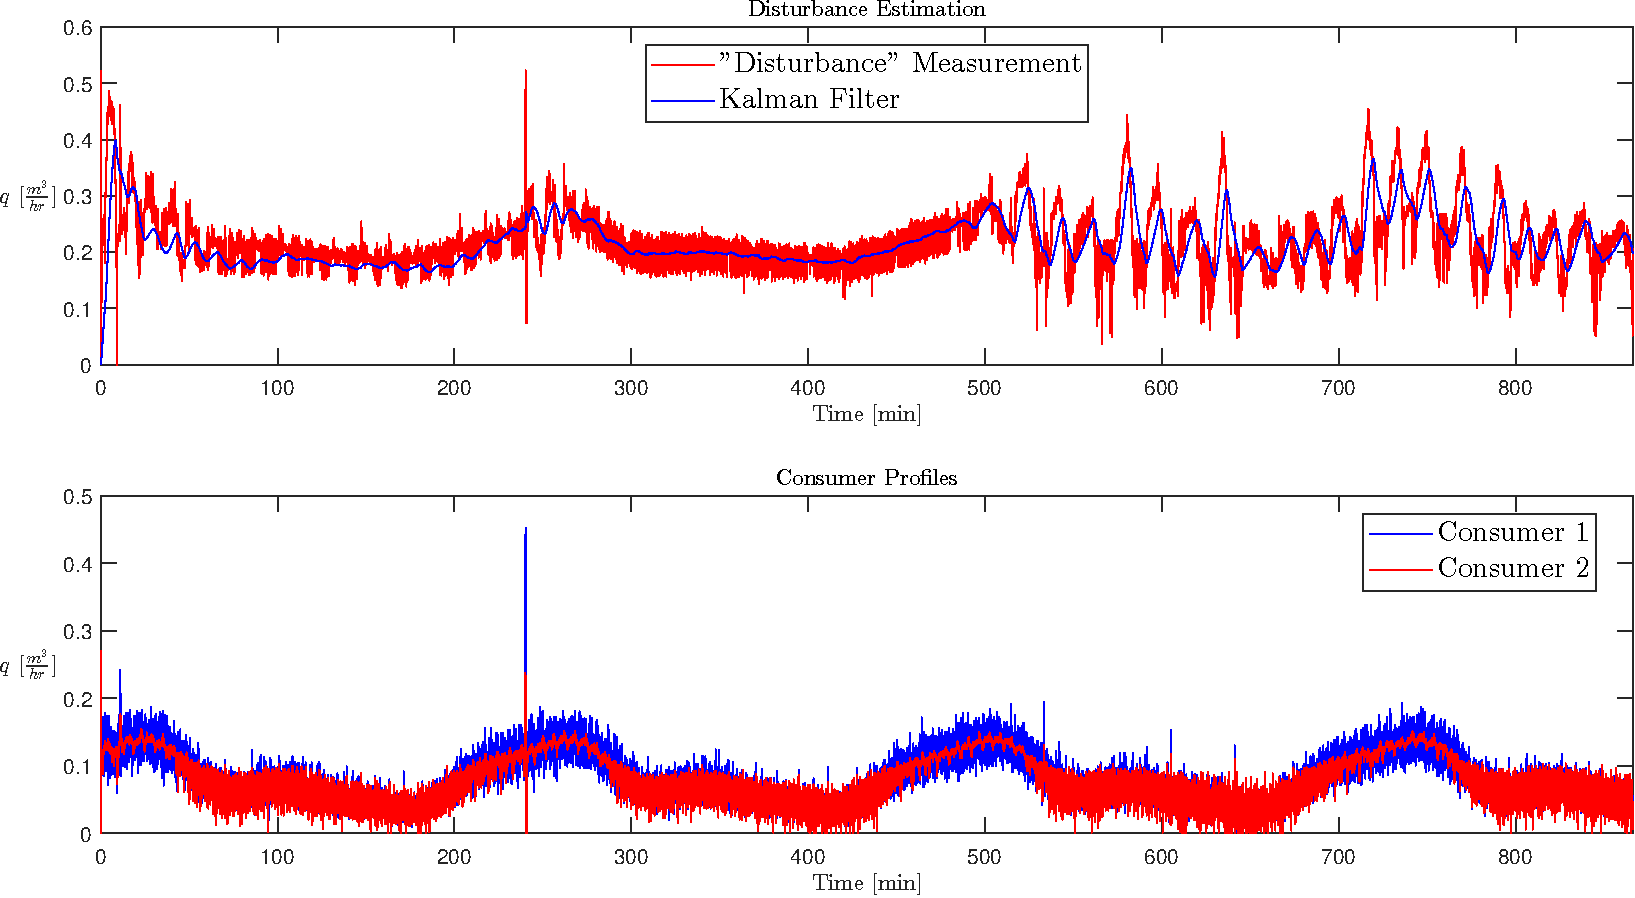
\includegraphics[height=4cm, width=\linewidth]{Graphics/DisturbanceEstimation.pdf}
	\caption{Consumer disturbance estimation.}
	\label{fig:DisturbanceEstimation}
\end{figure}

\begin{figure}[h!]
	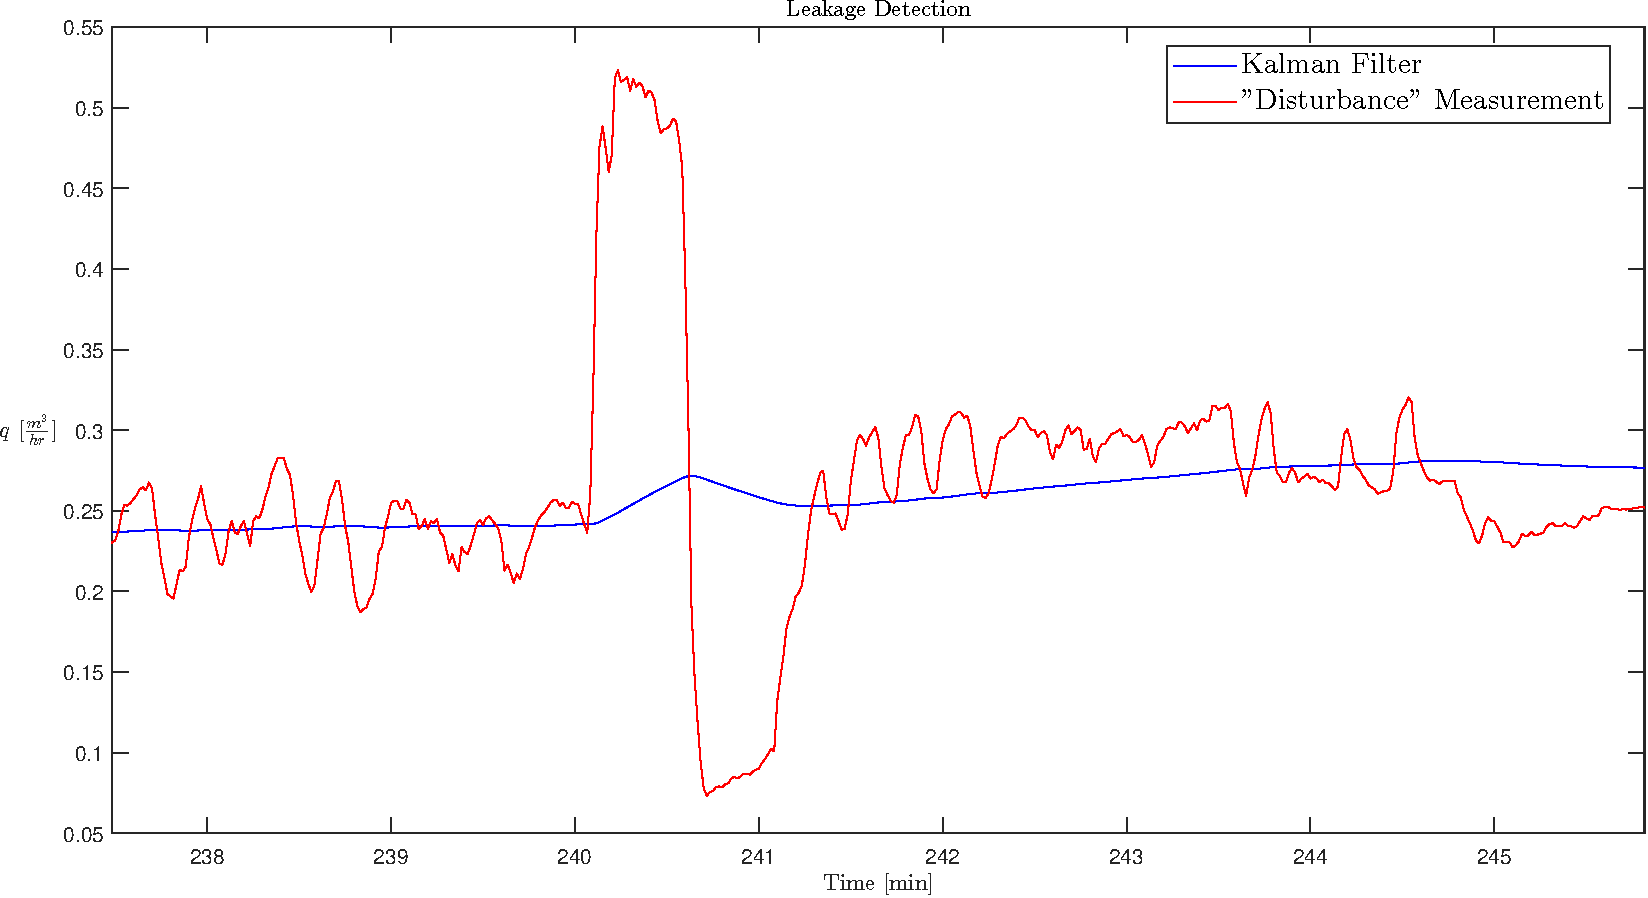
\includegraphics[height=4cm, width=\linewidth]{Graphics/LeakageDetection.pdf}
	\caption{Leakage detection.}
	\label{fig:Leakage}
\end{figure}



